\documentclass[letterpaper]{article}
\usepackage[thinlines]{easytable}
\usepackage{aaai20}
\usepackage{array}
\usepackage{times}
\usepackage{amsmath}
\usepackage{helvet}
\usepackage{courier}
\usepackage[hyphens]{url}
\usepackage{graphicx}
\usepackage[utf8]{inputenc}
\usepackage[portuguese]{babel} %separação silábica e outras coisas em português
\usepackage{bm} %negrito em math mode
\usepackage{icomma}
\urlstyle{rm}
\def\UrlFont{\rm}
\usepackage{graphicx}
\frenchspacing
\setlength{\pdfpagewidth}{8.5in}
\setlength{\pdfpageheight}{11in}

% Pacotes adicionais para tabelas e subfiguras, se necessário (verificar compatibilidade com aaai20)
\usepackage{booktabs} % Para tabelas mais bonitas
\usepackage{subcaption} % Para subfiguras

% PDFINFO
\pdfinfo{
/Title (Identificação dos Determinantes Socioeconômicos Mais Relevantes para Taxas de Suicídio Utilizando Aprendizado de Máquina)
/Author (Luan Pereira Pinheiro, Sofia Leopoldo)
/Keywords (Suicídio, Aprendizado de Máquina, Determinantes Socioeconômicos, ODS, Regressão Lasso, Árvores de Decisão)
}

\title{Identificação dos determinantes socioeconômicos mais relevantes para taxas de suicídio utilizando aprendizado de máquina}
\author{Luan Pereira Pinheiro\textsuperscript{\rm 1} e Sofia Leopoldo\textsuperscript{\rm 2}\\\\
Universidade de São Paulo, São Paulo, São Paulo, Brasil\\
\textsuperscript{\rm 1}13672471, \textsuperscript{\rm 2}14616969\\
\{\textsuperscript{\rm 1}luanpinheiro, \textsuperscript{\rm 2}sofialeopoldo\}@usp.br\\
}

\begin{document}
\maketitle

\begin{abstract}
Este artigo apresenta uma análise para identificar os determinantes socioeconômicos mais relevantes para as taxas de suicídio padronizadas por idade em diversos países, utilizando técnicas de aprendizado de máquina. Integrando dados em painel do \textit{World Development Indicators} (WDI) do Banco Mundial e da Organização Mundial da Saúde (OMS), o estudo emprega modelos de regressão, como Regressão Lasso e Árvores de Decisão, com foco em interpretabilidade. O pré-processamento envolveu uma seleção criteriosa de variáveis, tratamento de valores ausentes e mitigação da multicolinearidade. A metodologia culminou na identificação de um conjunto conciso de cinco indicadores socioeconômicos-chave. Os experimentos demonstraram que, apesar da complexidade do fenômeno, o modelo de Árvore de Decisão com esse conjunto reduzido alcançou um $R^2$ médio de 0{,}8234 e um RMSE de 8{,}56, enquanto o Lasso obteve $R^2$ de 0{,}2416 e RMSE de 36{,}82 — indicando que modelos baseados em árvores conseguem capturar não linearidades que a regressão linear não representa adequadamente. Os resultados revelam associações significativas, como o impacto da participação feminina na força de trabalho e do emprego industrial (ambos positivamente relacionados às taxas de suicídio), e, de forma protetiva, a densidade populacional, o acesso à eletricidade e o gasto privado com saúde. Essas descobertas contribuem para a formulação de políticas públicas mais eficazes na promoção da saúde mental e prevenção do suicídio, em consonância com os Objetivos de Desenvolvimento Sustentável (ODS) da ONU.
\end{abstract}
\section{Introdução} % Removido o asterisco

No ano de 2015 os 17 Objetivos de Desenvolvimento Sustentável (ODS) foram introduzidos à sociedade através da Agenda 2030, um plano de ações adotado internacionalmente para solucionar diversos problemas que afligem a população mundial ao mesmo tempo que reflete sobre questões ambientais e sustentabilidade. Os objetivos são estruturados em 17 categorias e metas específicas para uma delas, assim como parâmetros para avaliar a efetividade dos esforços coletivos de organizações de todo o mundo. Ainda assim, os objetivos são considerados muito ambiciosos e há grande preocupação acerca do cumprimento da agenda, uma vez que resta apenas um terço do prazo original: 5 anos \cite{unagenda2030}.

Entretanto, os 17 ODS e a Agenda 2030 são também uma referência para muitos outros projetos e planos de ações, concentrando grande atenção internacional para problemas chaves. Um exemplo de plano de ações desenvolvido com foco em uma das metas de ODS é o Plano de Ação Integral para a Saúde Mental, enquanto a saúde mental só está ativamente presente nas metas 3.4 e 3.5, sendo elas I. "Até 2030, reduzir em um terço a mortalidade prematura por doenças não transmissíveis via prevenção e tratamento, e promover a saúde mental e o bem-estar", II. "Reforçar a prevenção e o tratamento do abuso de substâncias, incluindo o abuso de drogas entorpecentes e uso nocivo do álcool", em que o segundo parâmetro definido para a primeira meta é a taxa de mortalidade por suicídio \cite{unagenda2030}.

\section{Arcabouço Teórico} % Removido o asterisco

O suicídio é um fenômeno sobre o qual diferentes ciências refletem com frequência, como por exemplo a filosofia e a psicologia, mas a sociologia também traz elementos indispensáveis para pensar o suicídio e a sua redução. O cientista social Émile Durkheim, considerado pai da sociologia, definiu em sua obra que o suicídio é uma questão social, e para entendê-la é necessário estudar não apenas fenômenos orgânico-psíquicos, mas também causas sociais. Isso se deu no contexto de transição do século XIX para o século XX, porém não poderia ser mais atual \cite{sociologia}.

De acordo com a Organização Mundial da Saúde, mais de 720 mil pessoas morrem todos os anos devido ao suicídio, sendo a terceira maior causa para o óbito de jovens entre 15 e 29 anos \cite{whosuicide}. A literatura também aponta que, a nível individual, homens tendem a cometer suicídio com maior frequência do que mulheres \cite{whosuicide_gender}.

Apesar de uma referência mundial, os 17 ODS frequentemente recebem críticas sobre a inclusividade. O próprio objetivo 3 não cita explicitamente o direito à saúde, o que reflete diretamente na consideração de fatores socioeconômicos e marginalização de um direito humano \cite{antiods}. Portanto, a investigação acerca desses fatores ainda é extremamente relevante.

Para isso, é interessante uma análise global do suicídio, e não apenas grupos focais. Dessa forma as questões socioeconômicas se revelam mais pertinentes e evita possíveis negligências a grupos marginalizadas, como povos indígenas. A definição de fatores socioeconômicos a partir de dados diversos é essencial para a efetividade de planos de ação combatentes do suicídio.

\section{Definição do problema} % Removido o asterisco
Ao longo deste artigo, realizaremos uma análise dos fatores socioeconômicos de diversos países para identificar os mais relevantes para a explicação das taxas de suicídio padronizadas por idade, utilizando técnicas de aprendizagem de máquina. Para isso, serão integrados dois conjuntos de dados distintos: o banco \textit{World Development Indicators} (WDI) \cite{wdi2024}, que reúne uma ampla gama de indicadores socioeconômicos de diversos países, e os dados da Organização Mundial da Saúde (OMS) com as taxas de suicídio padronizadas por idade, que serão utilizadas como variável alvo no modelo.

A análise será conduzida em um formato de dados de painel, onde cada observação representa um país em um determinado ano. Isso permite capturar variações tanto entre países quanto ao longo do tempo.

Apesar de o próprio conjunto de dados da WDI conter indicadores relacionados ao suicídio, opta-se pelo uso dos dados fornecidos pela OMS com padronização por idade, uma vez que essa abordagem corrige distorções demográficas e permite comparações mais justas entre diferentes países e ao longo do tempo. A taxa bruta de suicídio pode variar significativamente em função da estrutura etária da população, dado que a incidência de suicídio tende a ser maior em determinadas faixas etárias. Dessa forma, a padronização por idade elimina esse viés, proporcionando uma métrica mais confiável e comparável para análise \cite{whoageadjusted}.

A modelagem será conduzida com foco em interpretabilidade, permitindo identificar os fatores mais relevantes para seu aumento ou redução. Essa análise visa contribuir com a formulação de políticas públicas mais eficazes na promoção da saúde mental e na prevenção do suicídio.

\section{Metodologia} % Removido o asterisco
Para lidar com o problema definido, foi desenvolvido um sistema de aprendizado de máquina que utiliza os dados do WDI e da OMS para modelar as relações entre as variáveis socioeconômicas e as taxas de suicídio padronizadas por idade.

De modo geral, a solução implementada consistiu nas seguintes etapas: carregamento e integração dos dados das duas fontes; pré-processamento dos dados; modelagem preditiva utilizando algoritmos de aprendizado supervisionado; análise da importância das variáveis no modelo preditivo; e geração de um novo modelo, reaplicando o algoritmo com as variáveis mais relevantes identificadas.

\subsection{Carregamento e integração dos dados} % Removido o asterisco

Nesta etapa, os dados do WDI e as taxas de suicídio padronizadas por idade fornecidas pela OMS foram carregados. A aquisição dos dados da OMS foi feita a partir de um arquivo CSV, utilizando a base de dados completa disponível. Já a obtenção dos dados do WDI foi realizada programaticamente via API, utilizando paralelização de requisições para otimizar o tempo de coleta. Este processo de seleção inicial e automação da coleta foi conduzido com o auxílio do Gemini.

Inicialmente, o conjunto completo do WDI abrangia 1509 variáveis ao longo de 65 anos para 266 países. Devido às limitações de volume de download do WDI, tanto manual quanto via API, que impediam a obtenção de todo o conjunto de dados de uma só vez, foi essencial realizar uma seleção inicial de indicadores. Esta seleção, que resultou em 193 variáveis, excluiu aquelas menos prováveis de determinar causas de suicídio, os potencialmente correlacionados entre si ou com o suicídio sem indicar causa direta (e.g., outras taxas de mortalidade). Exemplos de variáveis removidas nesta etapa incluem indicadores muito específicos de negócios ("Bribery incidence", "Firms experiencing electrical outages"), dados ambientais detalhados ("Carbon dioxide (CO2) emissions", "PM2.5 air pollution"), métricas de desempenho de governança ("CPIA building human resources rating", "Control of Corruption: Estimate"), e outras taxas de mortalidade que, embora correlacionadas com o desenvolvimento socioeconômico, não representam causas diretas de suicídio ("Mortality rate, infant", "Mortality rate, under-5", "Intentional homicides").

O período de análise foi definido de 2000 a 2021, e o foco foi em 185 países que possuíam dados consistentes na base da OMS. A cobertura de países da base da OMS atuou como o gargalo para a integração, pois apenas os países presentes em ambas as bases e com dados consistentes puderam ser incluídos na análise final. Para garantir a correta associação entre as bases, foram utilizados os códigos ISO3 dos países (padrão internacional de três letras para identificação de países) como chave de integração, padronizando a nomenclatura entre os conjuntos de dados. As observações são tratadas a nível de país por ano, formando um painel de dados.

\subsection{Pré-processamento dos dados}

Dado o volume e a complexidade do conjunto de dados, um tratamento inicial rigoroso foi essencial. O processo de pré-processamento consistiu em várias etapas para lidar com dados faltantes e/ou redundantes.

O processo de pré-processamento e seleção de variáveis foi conduzido de forma iterativa, com o objetivo de reduzir a dimensionalidade do conjunto de dados, garantir a qualidade dos dados e preservar a interpretabilidade dos resultados. Inicialmente, o conjunto de dados continha 193 variáveis.

Como primeiro passo, foram excluídas as colunas com mais de 50\% de valores ausentes. A imputação de uma proporção tão elevada de dados poderia comprometer a validade das análises, introduzindo vieses e ruído, uma vez que a maior parte das informações seria artificialmente criada. Essa decisão se baseia em uma heurística comum em pré-processamento de dados, segundo a qual a confiabilidade da imputação se reduz significativamente com o aumento da proporção de dados faltantes \cite{chai2014rmse}. Após essa etapa, 48 variáveis foram descartadas, restando 145.

Em seguida, foi analisada a presença de variáveis com variância extremamente baixa, mas nenhuma apresentou variância inferior a 1\%, não havendo remoções nessa fase.

Após as remoções iniciais de colunas, observações (país-ano) com mais de 50\% de valores ausentes nas variáveis restantes foram eliminadas, resultando na exclusão de 114 linhas e um total de 3956 observações para a análise.

Com o conjunto reduzido, foi realizada uma análise de correlação entre as variáveis numéricas, utilizando a matriz de correlação absoluta. Para lidar com redundância entre variáveis altamente correlacionadas, construímos um grafo não-direcionado em que cada vértice representa uma variável, e adicionamos uma aresta entre dois vértices caso a correlação absoluta entre as variáveis fosse superior a 0{,}9. As componentes conexas desse grafo representam grupos de variáveis fortemente correlacionadas, e foram tratados como conjuntos para análise posterior.

Para cada componente com correlação mínima superior a 0{,}9, analisamos qualitativamente qual variável era mais interpretável, considerando critérios como clareza conceitual, relevância socioeconômica e formato dos dados (preferência por variáveis per capita, estimativas em vez de percentis, e medidas agregadas em detrimento de segmentadas). Dentro de cada conjunto, removemos as variáveis menos interpretáveis ou com menor cobertura, mantendo apenas uma por conjunto. Em casos de empate em interpretabilidade e cobertura, a variável com menor variância foi removida, uma vez que baixa variância reduz a capacidade discriminativa do modelo. Após esse processo, restaram 82 variáveis.

Ainda com base na estrutura de componentes correlacionados, identificamos oito variáveis adicionais cuja presença era redundante. Nesse momento, o grafo possui apenas componentes conectados cuja mínima correlação entre dois vértices é menor que 0{,}9. Para realizar essa filtragem final de forma sistemática, consideramos novamente o grafo de variáveis com correlação acima de 0{,}9, e buscamos um conjunto independente máximo (maximum independent set, MIS) \cite{west2001introduction}, ou seja, um subconjunto de variáveis não correlacionadas entre si, mas representando toda a estrutura do grafo com o mínimo de sobreposição. Essa abordagem é adequada para manter a diversidade informacional sem redundância, especialmente quando já se garantiu a interpretabilidade das variáveis restantes.

A aplicação do MIS levou à exclusão final de oito variáveis altamente correlacionadas entre si, totalizando 74 variáveis ao fim do processo.

Os valores ausentes remanescentes nessas 74 variáveis foram imputados utilizando a mediana de cada coluna — uma abordagem simples, robusta e menos sensível a \textit{outliers}. 

\subsection*{Modelagem preditiva} % Alterado para subseção sem número
Como o objetivo do projeto é encontrar as variáveis socioeconômicas que mais contribuem para explicar as taxas de suicídio, a modelagem preditiva foi conduzida com foco em interpretabilidade. Para isso, foi realizada uma comparação entre dois algoritmos de aprendizado de máquina: regressão Lasso (\textit{Least Absolute Shrinkage and Selection Operator}) e árvores de decisão.

A regressão Lasso é uma técnica de regressão linear com regularização L1, que tende a atribuir zero para variáveis menos relevantes, promovendo seleção automática de atributos \cite{tibshirani1996regression}, sendo, portanto, muito adequada ao nosso problema.

As árvores de decisão, por outro lado, permitem capturar relações não lineares entre as variáveis e a variável alvo, além de fornecer métricas claras de importância dos atributos com base na redução de impureza em cada divisão \cite{breiman1986classification}. Para problemas de regressão, a árvore busca minimizar o Erro Quadrático Médio (MSE) em cada nó, e a previsão final para um novo dado é a média dos valores da variável alvo nos nós folha.

A escolha desses dois algoritmos visou explorar abordagens complementares — uma linear e outra não linear — para garantir maior robustez na identificação das variáveis mais relevantes e avaliar a estabilidade dos resultados obtidos.

A análise da importância das variáveis foi realizada com base nos coeficientes da regressão Lasso e nas taxas de importância (\textit{feature importance scores}) extraídas diretamente do modelo de árvore de decisão. Esses critérios permitiram identificar quais indicadores do WDI estão mais associados às variações nas taxas de suicídio padronizadas por idade.

Em seguida, foi gerado um novo modelo com as variáveis mais relevantes identificadas, de modo a investigar a viabilidade de reduzir a dimensionalidade sem comprometer o desempenho preditivo.

\section{Metodologia de avaliação} % Removido o asterisco
Para avaliar a performance dos modelos gerados, foi adotada a técnica \textit{r-fold cross-validation}, de forma a garantir robustez na avaliação.

As métricas selecionadas para a avaliação e comparação dos modelos finais são:

\begin{itemize}
    \item \textbf{Raiz Quadrada do Erro Quadrático Médio (RMSE)}: métrica que mede a média dos erros quadráticos entre os valores previstos e os reais. Penaliza mais fortemente grandes erros e é útil quando erros maiores são mais indesejáveis \cite{chai2014rmse}.
    \item \textbf{Coeficiente de Determinação ($R^2$)}: mede a proporção da variabilidade da variável dependente que é explicada pelo modelo. Um valor de $R^2$ próximo de 1 indica bom ajuste, enquanto valores próximos de 0 indicam baixa capacidade explicativa \cite{frost2019r2}.
\end{itemize}

Para fenômenos sociais complexos como o suicídio, que são influenciados por múltiplos fatores — não apenas socioeconômicos —, valores de $R^2$ moderados (entre 0{,}30 e 0{,}70) podem ainda assim indicar uma capacidade explicativa relevante no contexto das ciências sociais \cite{soc_r2_interpretation}. Cohen (1992) considera efeitos com $R^2$ a partir de 0{,}26 como grandes em estudos comportamentais, o que reforça a relevância de modelos com esse nível de ajuste mesmo diante da complexidade do fenômeno.

\section{Experimentos}

A comparação entre os modelos de Regressão Lasso e Árvores de Decisão demonstrou uma vantagem clara do segundo em termos de desempenho preditivo. Como mostram as métricas a seguir, a Árvore de Decisão alcançou valores de $R^2$ e erro quadrático médio significativamente melhores em relação ao Lasso:

\vspace{0.5em}
\noindent
\textbf{Métricas iniciais da Árvore de Decisão:}
\begin{itemize}
\item $R^2$ médio: 0.8617 ($\pm$ 0.0166)
\item MSE médio: 6.71 ($\pm$ 0.77)
\end{itemize}

\noindent
\textbf{Métricas iniciais do Lasso:}
\begin{itemize}
\item $R^2$ médio: 0.3811 ($\pm$ 0.0155)
\item MSE médio: 30.06 ($\pm$ 1.08)
\item Melhor $\alpha$: 0.0135
\end{itemize}

\vspace{0.5em}

Essa diferença de desempenho é esperada, dado que as Árvores de Decisão conseguem capturar relações não lineares e interações entre variáveis, enquanto a regressão Lasso assume uma relação linear entre as variáveis explicativas e a variável dependente.

As Figuras \ref{fig:comparacao_r2} e \ref{fig:comparacao_mse} também permitem ver a discrepância entre os erros da Regressão Lasso e da Árvore de Decisão. Dada essa diferença substancial, optamos por usar a Árvore de Decisão como base principal para a seleção de variáveis relevantes, priorizando aquelas com boa capacidade explicativa e com interpretações alinhadas com a literatura.

\begin{figure}[h]
    \centering
    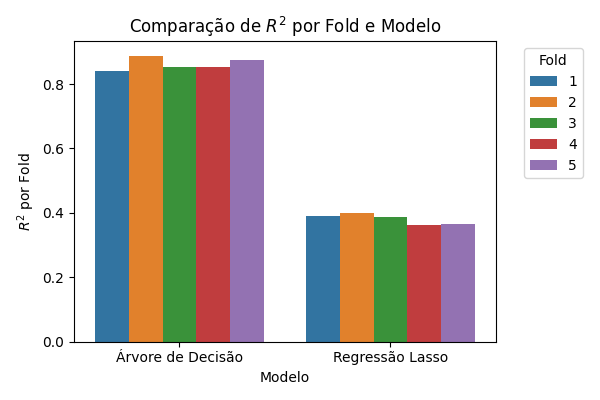
\includegraphics[width=0.5\textwidth]{comparacao_r2_modelos.png}
    \caption{Comparação do $R^2$ por fold entre os modelos de Regressão Lasso e Árvore de Decisão.}
    \label{fig:comparacao_r2}
\end{figure}

\begin{figure}[h]
    \centering
    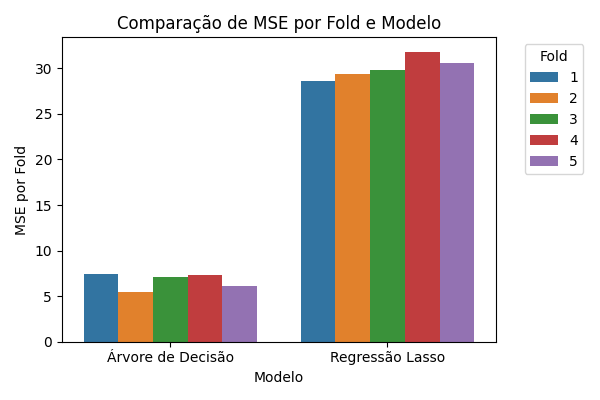
\includegraphics[width=0.5\textwidth]{comparacao_mse_modelos.png}
    \caption{Comparação do MSE por fold entre os modelos de Regressão Lasso e Árvore de Decisão.}
    \label{fig:comparacao_mse}
\end{figure}

Além da importância de cada variável (fornecida pelo modelo de árvore), nosso programa também avaliou a direcionalidade da associação: se o aumento da variável tende a aumentar ou diminuir as taxas de suicídio previstas. Isso foi feito analisando a proporção de divisões positivas e negativas na árvore, bem como a proporção de amostras afetadas por cada tipo de divisão. As variáveis que apresentaram relações claras e consistentes com o suicídio — seja positiva ou negativa — foram priorizadas, enquanto variáveis com comportamento ambíguo ou contraintuitivo foram descartadas.

A Tabela \ref{tab:final_features} apresenta o conjunto final de 5 variáveis selecionadas após múltiplas iterações com o modelo de árvore e refinamentos manuais voltados à interpretabilidade. Incluímos a importância relativa, a direção da associação observada e uma justificativa qualitativa baseada na literatura.


\begin{table*}[ht]
\centering
\caption{Variáveis Socioeconômicas Selecionadas e Sua Associação com as Taxas de Suicídio}
\label{tab:final_features}
\renewcommand{\arraystretch}{1.4}
\begin{tabular}{>{\raggedright\arraybackslash}p{0.35\textwidth} 
                >{\centering\arraybackslash}p{0.1\textwidth} 
                >{\centering\arraybackslash}p{0.2\textwidth} 
                >{\raggedright\arraybackslash}p{0.25\textwidth}}
\toprule
\textbf{Variável (Indicador WDI)} & \textbf{Importância} & \textbf{Direção da Associação} & \textbf{Interpretação} \\
\midrule
Labor force, female (\% of total labor force) & 0.296 & Maior $\rightarrow$ Maior taxa & Estresse por “dupla jornada” \\
Population density (people per sq. km of land area) & 0.284 & Maior $\rightarrow$ Menor taxa & Acesso a serviços, redes sociais \\
Employment in industry (\% of total employment) (modeled ILO estimate) & 0.169 & Maior $\rightarrow$ Maior taxa & Estresse e instabilidade em ambientes industriais \\
Access to electricity (\% of population) & 0.137 & Maior $\rightarrow$ Menor taxa & Indicador de desenvolvimento e qualidade de vida \\
Domestic private health expenditure per capita, PPP (current international \$) & 0.115 & Maior $\rightarrow$ Menor taxa & Maior acesso a serviços de saúde, incluindo saúde mental \\
\bottomrule
\end{tabular}
\end{table*}

\subsection*{Discussão dos Determinantes Chave}

\begin{itemize}
\item \textbf{Participação Feminina na Força de Trabalho:} A variável \textit{Labor force, female} apresentou a maior importância no modelo (0.296). Cerca de 69.1\% das amostras impactadas por essa variável resultaram em previsões maiores de suicídio. A literatura sugere que esse padrão pode estar relacionado ao acúmulo de responsabilidades e ao estresse enfrentado por mulheres em contextos onde se espera que conciliem trabalho formal e cuidado doméstico \cite{female_labor_force_impact_stack}.

\item \textbf{Densidade Populacional e Acesso a Serviços:} As variáveis \textit{Population density}, \textit{Access to electricity} e \textit{Domestic private health expenditure per capita} apresentaram importâncias de 0.284, 0.137 e 0.115, respectivamente. Para \textit{Population density}, 61.9\% das amostras afetadas levaram a predições de menor suicídio. Para \textit{Access to electricity}, essa proporção foi de 76.6\%, e para \textit{Private health expenditure}, 65.2\%. Esses dados sugerem que a urbanização e o maior acesso à infraestrutura básica e serviços de saúde — inclusive mental — atuam como fatores de proteção, o que é suportado pela literatura \cite{kegler2017trends}.

\item \textbf{Estrutura Econômica:} A variável \textit{Employment in industry} teve importância de 0.169, com 66.2\% das amostras associadas a ela resultando em aumentos nas predições de suicídio. Esse achado pode refletir condições adversas de trabalho em ambientes industriais, como tarefas repetitivas, baixo controle sobre o processo de trabalho e altos níveis de estresse ocupacional. A prevalência de suicídio maior entre empregados industriais é um fato conhecido \cite{sussell2023suicide}
\end{itemize}

Para avaliar a robustez do modelo com esse conjunto reduzido de variáveis, reestimamos o desempenho da Árvore de Decisão, que manteve resultados satisfatórios:

\vspace{0.5em}
\noindent
\textbf{Métricas com conjunto reduzido (Árvore de Decisão):}
\begin{itemize}
\item $R^2$ médio: 0.8234 ($\pm$ 0.0271)
\item MSE médio: 8.56 ($\pm$ 1.17)
\end{itemize}

Também testamos a regressão Lasso com as mesmas cinco variáveis, com desempenho inferior, mas ainda relevante:

\vspace{0.5em}
\noindent
\textbf{Métricas com conjunto reduzido (Regressão Lasso):}
\begin{itemize}
\item $R^2$ médio: 0.2416 ($\pm$ 0.0145)
\item MSE médio: 36.82 ($\pm$ 1.08)
\end{itemize}

Esses resultados reforçam que é possível utilizar um conjunto pequeno e interpretável de variáveis socioeconômicas para explicar variações nas taxas de suicídio, mantendo bom desempenho preditivo e facilitando a análise de políticas públicas.

\section{Conclusão}

Este estudo utilizou técnicas de aprendizado de máquina para identificar os determinantes socioeconômicos mais relevantes para as taxas de suicídio padronizadas por idade em uma análise de painel de dados entre países. Através de um rigoroso processo de pré-processamento e seleção de variáveis, foi possível construir um modelo interpretável que destaca cinco fatores-chave.

Os resultados apontam para a complexidade das relações entre fatores socioeconômicos e o suicídio, revelando associações que, embora por vezes contraintuitivas à primeira vista, são apoiadas por literatura especializada (e.g., o papel da participação feminina na força de trabalho). Indicadores de desenvolvimento, acesso a serviços e estabilidade econômica geral foram consistentemente associados a menores taxas de suicídio.

\textbf{Limitações e Trabalhos Futuros:} As limitações deste estudo incluem a natureza agregada dos dados, que impede conclusões sobre causalidade em nível individual (falácia ecológica). Além disso, a disponibilidade de dados para alguns indicadores e países pode ter influenciado a seleção final de variáveis. Nenhuma tupla no conjunto original continha todas as variáveis simultaneamente, exigindo a imputação de dados em todos os casos — o que pode ter introduzido ruído ou padrões artificiais. O critério adotado para reter variáveis com até 50\% de valores ausentes pode ter sido permissivo, comprometendo parcialmente a qualidade do modelo.

Adicionalmente, a direcionalidade das associações entre variáveis e taxas de suicídio foi inferida com base em uma heurística empírica: analisou-se a proporção de divisões positivas e negativas nas árvores de decisão, bem como a proporção de amostras afetadas. Embora essa abordagem tenha oferecido uma visão inicial útil, estudos futuros poderiam empregar técnicas mais robustas e bem fundamentadas, como LIME ou SHAP, para estimar a influência local e global das variáveis com maior precisão e confiabilidade.

Trabalhos futuros também poderiam explorar a investigação de como a importância e a direcionalidade desses determinantes variam em diferentes contextos culturais e políticos, por exemplo, usando as regiões definidas pela OMS ou as faixas de renda definidas pelo Banco Mundial.

A compreensão desses determinantes é fundamental para o desenvolvimento de políticas públicas mais eficazes e direcionadas à promoção da saúde mental e à prevenção do suicídio, contribuindo para o avanço dos Objetivos de Desenvolvimento Sustentável da ONU.

\bibliographystyle{aaai}
\bibliography{bibfile}

\end{document}

